% mnras_template.tex
%
% LaTeX template for creating an MNRAS paper
%
% v3.0 released 14 May 2015
% (version numbers match those of mnras.cls)
%
% Copyright (C) Royal Astronomical Society 2015
% Authors:
% Keith T. Smith (Royal Astronomical Society)

% Change log
%
% v3.0 May 2015
%    Renamed to match the new package name
%    Version number matches mnras.cls
%    A few minor tweaks to wording
% v1.0 September 2013
%    Beta testing only - never publicly released
%    First version: a simple (ish) template for creating an MNRAS paper

%%%%%%%%%%%%%%%%%%%%%%%%%%%%%%%%%%%%%%%%%%%%%%%%%%
% Basic setup. Most papers should leave these options alone.
\documentclass[fleqn,usenatbib]{mnras}  % a4paper,

% MNRAS is set in Times font. If you don't have this installed (most LaTeX
% installations will be fine) or prefer the old Computer Modern fonts, comment
% out the following line
%\usepackage{newtxtext,newtxmath}
%\usepackage{lmodern}
% Depending on your LaTeX fonts installation, you might get better results with one of these:
\usepackage{mathptmx}
%\usepackage{txfonts}


% Use vector fonts, so it zooms properly in on-screen viewing software
% Don't change these lines unless you know what you are doing
\usepackage[T1]{fontenc}
\usepackage{ae,aecompl}
\usepackage{slashbox}

%%%%% AUTHORS - PLACE YOUR OWN PACKAGES HERE %%%%%

% Only include extra packages if you really need them. Common packages are:
\usepackage{graphicx}	% Including figure files
\usepackage{amsmath}	% Advanced maths commands
\usepackage{amssymb}	% Extra maths symbols
\usepackage{savesym}  % prevent symbol conflicts
\savesymbol{sf}
%\generate{%
%  \file{breqn.sty}{\nopreamble\from{breqn.dtx}{breqn.sty}}%
%}
%\usepackage{breqn} % automatic breaking equation 
%\usepackage{fancyvrb}
%\VerbatimFootnotes
\usepackage{cprotect}  % to allow verb in caption 
\DeclareMathOperator\erfc{erfc}
\DeclareMathOperator\erf{erf}
\DeclareMathOperator\cdf{cdf}
\DeclareMathOperator\sf{sf}
\DeclareMathOperator\isf{isf}
\DeclareMathOperator\ppf{ppf}

%%%%%%%%%%%%%%%%%%%%%%%%%%%%%%%%%%%%%%%%%%%%%%%%%%

%%%%% AUTHORS - PLACE YOUR OWN COMMANDS HERE %%%%%

% Please keep new commands to a minimum, and use \newcommand not \def to avoid
% overwriting existing commands. Example:
%\newcommand{\pcm}{\,cm$^{-2}$}	% per cm-squared

%%%%%%%%%%%%%%%%%%%%%%%%%%%%%%%%%%%%%%%%%%%%%%%%%%

%%%%%%%%%%%%%%%%%%% TITLE PAGE %%%%%%%%%%%%%%%%%%%

% Title of the paper, and the short title which is used in the headers.
% Keep the title short and informative.
\title[SDSS Quasars]{SDSS Stripe 82 : quasar variability from forced photometry}

% The list of authors, and the short list which is used in the headers.
% If you need two or more lines of authors, add an extra line using \newauthor
\author[K. Suberlak et al.]{
Krzysztof Suberlak,$^{1}$\thanks{E-mail: suberlak@uw.edu}
\v{Z}eljko Ivezi\'c, $^{1}$
Yusra AlSayyad,$^{1}$ 
\\
% List of institutions
$^{1}$Department of Astronomy, University of Washington, Seattle, WA, United States\\
}

% These dates will be filled out by the publisher
\date{Accepted XXX. Received YYY; in original form ZZZ}

% Enter the current year, for the copyright statements etc.
\pubyear{2015}

% Don't change these lines
\begin{document}
\label{firstpage}
\pagerange{\pageref{firstpage}--\pageref{lastpage}}
\maketitle

% Abstract of the paper
\begin{abstract}

\end{abstract}


%%%%%%%%%%%%%%%%%%%%%%%%%%%%%%%%%%%%%%%%%%%%%%%%%%

%%%%%%%%%%%%%%%%% BODY OF PAPER %%%%%%%%%%%%%%%%%%

\section{Introduction}
\label{sec:intro}
Many objects in the universe, from stellar to extragalactic scales, vary on timescales less than a few hundred years. Lightcurves carry a wealth of information allowing one to infer various physical properties of a planet or a galaxy. If a lightcurve is poorly sampled, the inferred  characteristics are less certain. Yet, since all  astronomical observations suffer from a detection threshold, a very faint variable object in some epochs may be undetectable. Forced photometry rescues the information from very faint epochs by performing a measurement in all epochs in a location from the co-added images. An inherent challenge to such set of measurements is an intepretation of noise-dominated flux. To circumvent this problem many studies apply a magnitude cutoff few magnitudes above the detection limit, which reduces the amount of available data. Indeed, in order to fully utilize information present in time-domain surveys, such as Large Scale Synoptic Telescope, Palomar Transient Factory, or Sloan Digital Sky Survey, and properly characterize faint variable objects, we need to properly handle the faint flux measurements. A new methodology would allow an unbiased  study of such faint variable objects, including quasars,  RR Lyrae,  Cepheids, and a wealth of other variable sources.  With the advent of precision  time-domain astronomy  surveys it is crucial to apply the best possible faint forced photometry algorithms and thus make full use of the  data.  

\section{Methods}


\subsection{Data Overview}
\label{sec:data}
\subsubsection{Stripe 82}
We use data from all SDSS runs up to an including run 7202 (Data Release 7), including all 6 SDSS camera columns. Stripe 82 survey covered an equatorial strip of the sky, defined by declination limits of $\pm1.27\deg$, extending from R.A. $\approx$ $20^{h} (320 \deg)$ to R.A.  $\approx$ $4^{h} (55 \deg)$ (Sesar+2010). Observations conducted prior to September 2005 (part of SDSS I-II) had a more sparse sampling than SDSS-III, and the SDSS Supernova Survey, which ran between September 1st - November 30th each year between 2005-2007. 

The SDSS Stripe 82 DR7  data  was processed in two data centers : NCSA (National Center for Supercomputing Applications, University of Illinois at Urbana-Champaign, IL) and IN2P3  (Institut national de physique nucl\'eaire et de physique des particules in Paris, France). NCSA processed data from $-40 \deg \, (+320 \deg) < RA < +10 \deg $ and IN2P3 with $ +5 \deg < RA < +55 \deg$ . There is a $5 \deg$ overlap, used to confirm that the data processing pipeline in both data centers yields identical data products. The entire strip was split into smaller patches

All epochs (individual images) were background-subtracted, and then scaled from the Digital Unit counts to fluxes by comparing standard objects against the Ivezic+2007 catalog  (similar to  Jiang+2014).   

\subsubsection{Source Detection}
Sources were detected in the i-band coadds. Each detection in the coadded images was assigned a deepSourceId (elsewhere called objectId). Considering  a dense region with clumped stars and/or galaxies, the entire clump was considered as one parent source (with single ParentSourceId). For an object which is a parent (eg. a galaxy), ParentSourceId is null. Solitary sources which are not blended  in clumps are their own parents. The result of this procedure were $~40$ million  i-band detections down to $3 \, \sigma$.  $8$ million of those are brighter than $23^{rd}$ mag. Part of Stripe82 processed in NCSA yielded  $20978391$ detections (\verb|iCoaddAll.csv|). The part that does not overlap with IN2P3 has   $16520093$ sources (\verb|iCoaddPhotometryAll.csv|), of which  $16514187$ are brighter than $30^{mag}$  ($5906$ less) (\verb|DeepSourceNCSA_i_lt300.csv|).

\subsubsection{Forced Photometry}
On positions specified by the detection data AlSayyad+2015 performed forced photometry in all SDSS photometric bands, on the individual epoch images. It is different from image differences technique, where the photometry is done on a difference between a coadd and an individual epoch image.  The total number of photometric measurements (combining NCSA and IN2P3) was  ($40$  million i-band detections) x ($80$ epochs ) x ($5$ filters) = $~16$ billion measurements, including   ($8$ million i-band detections i < 23) x ($80$ epochs) x ($5$ filters ) = $3.2$ billion measurements brighter than $23^{rd}$ mag.
For each patch the raw lightcurves contain the \verb|id|, \verb|objectId|, \verb|exposure_id|, \verb|mjd|, \verb|psfFlux|, \verb|psfFluxErr|, sorted by \verb|objectId|, measuring flux in $[ergs/ cm^{2} / sec / Hz]$ (\verb|rawDataFPSplit/bandPatchStart_PatchEnd.csv|). 



\subsection{Analysis}

\subsubsection{Faint Sources}
\label{sec:faint_sources}

%
%%%%%%%%%%%%%%%%% MOTIVATION %%%%%%%%%%%%%%%%%
%
Forced photometry in a background-subtracted epoch may yield unphysical, negative values. Such negative pixel value may originate from the variation of background across the image. If we model the background counts  as a Gaussian centered around the mean  $B_{0}$ :   $B-B_{0}  \sim  \mathcal{N}(0,\sigma_{B})$, then background in some parts of the image will be above, and in other parts below the mean value. After subtraction of the mean background value, regions with previously lower than average background will have negative pixel value.  This means that a forced photometry on a location where an object is undetected in single epoch may be measuring the background noise. Apart from creating low pixel values, background oscillation may also cause spurious detections where it is above the mean. For a large number of photons hitting the detector the width of the background noise distribution is  proportional to the square-root of counts: $\sigma_{B} \propto \sqrt {B}$. This yields a 1 in a million chance that a pixel has a background value larger than $5\sigma_{B}$.   Thus on a 16 megapixel CCD, like those used in SDSS, we anticipate  about  16 spuriously bright pixels  per CCD.  Therefore,  since forced photometry is affected by  the background noise, a special care must be taken of faint, noise-dominated measurements. 

%
%%%%%%%%%%%%%%%%% TREATMENT %%%%%%%%%%%%%%%%%
%

We remedy the unphysically low, even negative measurements for all 'faint' ($< 2\sigma$) sources and recalculate their fluxes. Each flux measurement can  be thought of as a  mean of the 'intrinsic' flux likelihood function $L(F)$. $L$ determines the probability that the flux has a value $F$. In our treatment we assume that $L$ is a Gaussian, and therefore its width corresponds to the measurement error :  $L(F) \sim \mathcal{N}(F,\sigma_{F})$. This means that bright sources with high signal-to-noise ratio have very narrow  $L$, and faint sources, dominated by noise, have $L$ with very wide tails.  Only for faint sources a significant portion of $L$ may be negative, corresponding to non-zero likelihood of flux being negative. This stands in conflict with our prior knowledge that no physical flux can be negative. We resolve this problem by recalculating single-epoch flux for all sources where $F < 2 \sigma_{F}$. We calculate for each epoch the mean of the truncated $L$, such that $L(F) = 0$ for $F<0$.  This shifts upward all measurements for faint epochs, and remedies the unphysicality of faint forced photometry fluxes.   

%
%%%%%%%%%%%%%%%%% CHOICE OF PRIOR %%%%%%%%%%%%%%%%%
%

In our treatment we are explicitly using a prior understanding of the flux behavior of any astrophysical object.  Without any further knowledge about the nature of the source, flat prior is the least informative Bayesian prior. Any additional information about the nature of object, and thus expected variability pattern,  could affect the choice of prior to be more specific. For instance,  consider a sinusoidal flux variability. If the flux of an object over many epochs is expected to vary in a sinusoidal fashion, i.e. $F(t) = F_{min}+ sin(t)$, the probability of a given  flux measurement is a cosine, ranging from $F_{min}$ to $F_{max}$. With that prior, without any measurement taken, the flux of the object is most likely  $(F_{min} + F_{max}) /  2$, i.e. at the peak of the cosine likelihood function. However, as soon as one measures $(F_{i},e_{i})$ from that source, the probability distribution of a flux at that epoch becomes a convolution of cosine prior information with the Gaussian curve of width $e_{i}$, centered on $F_{i}$ (assuming Gaussian errors). However, without any a-priori information about the variability pattern of the considered object, the least informative Bayesian prior we can impose is a flat one : $p(F)=0 $ for $F<0$, and $1$ elsewhere. Thus the posterior probability is 

\begin{equation}
p(F|data) \propto L(F|data) p(F)
\end{equation}


%
%%%%%%%%%%%%%%%%% WHAT WE CALCULATE %%%%%%%%%%%%%%%%%
%

To test the method we generate fiducial lightcurves (DRW / sinusoidal), with a uniform sampling ($N=100\div1000$). Based on the generated flux ($F_{true}$) we define the $5\sigma$ level as the robust 25-th percentile (or median) of the ensemble $F_{true}$ distribution :  $\sigma_{F} = (1/5)  F_{25 \%}$ (in reality, $\sigma$ increases for fainter observations, but this is a good approximation). 
\newline
We define $F_{obs} = F_{true} + F_{noise}$, where the Gaussian noise $F_{noise} = \sigma_{F}  \, \mathcal{N}(0,1)$ was added to each point. 
For a weak signal, defined as $F_{obs}^{i} < 2 \sigma{F}$, we consider $p(F)$  - a  Gaussian  likelihood associated with $i$-th measurement: $p_{i}(F) = \mathcal{N}(\mu=F_{obs}^{i}, \sigma=\sigma_{F})$. Each measurement $F_{obs}$ is a mean of this likelihood: $F_{obs} = \langle p_{i}(F) \rangle$. We call it $p(F)$  for short : 



For each epoch, based on the raw forced photometry measurement, we calculate new descriptors of faint fluxes. We define a faint measurement by $F_{i} < 2 \sigma{F_{i}}$, i.e. where the flux is less than twice the flux error. We assume that the flux is the mean of the Gaussian likelihood  $p_{i}(F) = \mathcal{N}(\mu=F_{i}, \sigma=\sigma_{F_{i}})$ : 
\begin{equation}
p(F) = \frac{1}{\sqrt{2  \pi \sigma_{F}^{2}}} \exp{ \left(-\frac{(F-\mu)^{2}}{2\sigma_{F}^{2}}\right)}
\end{equation}

so that $F_{i} =\langle p(F) \rangle $.  For faint measurements we truncate the negative part of $p(F)$, and recalculate the mean, median, rms, and $2 \sigma$ level. Thus the mean is  


\begin{equation}
F_{mean} = \frac{\int _{0} ^ {\infty}{F p(F) dF}}{\int _{0} ^ {\infty}{p(F) dF}}
\end{equation} 
where we normalized the truncated Gaussian likelihood.
 
We define the median as  

\begin{equation}
\int _{0} ^ {F_{median}} {p(F) dF} = \int _{F_{median}} ^ {\infty} {p(F) dF}
\end{equation} 

The rms level is

\begin{equation}
F_{rms}^{2} = \frac{\int _{0} ^ {\infty}{(F-F_{mean})^{2} p(F) dF}}{\int _{0} ^ {\infty}{p(F) dF}} 
\end{equation}

Finally, since for a Gaussian distribution the area contained between $\mu \pm \sigma$ is $95.5 \%$ of the total area under the curve, for the truncated Gaussian we define the  $2 \sigma$ level as:

\begin{equation}
\int _{F_{2 \sigma}} ^{\infty} {p(F)dF} = 0.05 * \int _{0} ^{\infty} {p(F) dF} 
\end{equation}

Both for median and for the $2\sigma$ level the normalization cancels out. For details, see Appendix ... 


\subsubsection{Variability}


%
%%%%%%%%%%%%%%%%% MOTIVATION %%%%%%%%%%%%%%%%%
%

%\subsubsection{Lightcurve statistics}

%
%%%%%%%%%%%%%%%%% STATISTICS WE USE %%%%%%%%%%%%%%%%%
%
%
%  STANDARD ONES 
%
In what follows, for faint measurements we choose to replace $F$ with $F_{mean}$. For all objects we calculate statistics based on entire lightcurves. We denote $(F_{obs}, \sigma_{obs})$ as $(x_{i},\sigma_{i})$ : 

- mean weighted by  $w_{i} = (\sigma_{i})^{-2}$
%\begin{gather*}
\begin{equation}
%\begin{align}
\bar{x} = \frac{\sum_{i=1}^{N}{w_{i}x_{i}}}{\sum_{i=1}^{N}{w_{i}}}
%\end{align}
\end{equation}
%\end{gather*}

- weighted mean error 
\begin{equation}
\sigma_{\bar{x}} = \left( \sum{w_{i}}\right) ^{-1/2} 
\end{equation}

- weighted standard deviation 
\begin{equation}
\sigma_{st.dev.w.} = \left( \frac{\sum{w_{i}(x_{i} - \bar{x})^{2}}}{\frac{N-1}{N}\sum{w_{i}}} \right) ^ {1/2}
\end{equation}

- error on standard deviation 
\begin{equation}
\sigma_{s} = \frac{1}{\sqrt{2}}\sqrt{\frac{N}{N-1}} \sigma_{\bar{x}}
\end{equation}

- robust interquartile width
\begin{equation}
\sigma_{G} = 0.7414 * (75\% - 25\%) 
\end{equation}

- median as the 50-th percentile , median error 
\begin{equation}
\sigma_{median} = \sqrt{\pi/2}\sigma_{\bar{x}}
\end{equation}
 

%- skewness 

%\begin{figure}
%\label{fig:sim_lc}
% 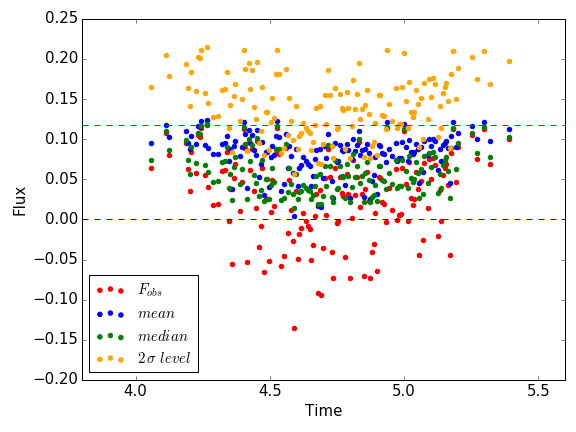
\includegraphics[width=\columwidth]{Flux_exp_faint.png}
%\caption{A portion of a simulated lightcurve with arbitrary time and flux units, where the simulated forced photometry flux is below the 2 sigma %%level. The simulated observed points that are below 2 sigma level,  may even drop below zero, and  are subjected to our algorithm correctiong for the unphysicality of such situation. Thus we impose the non-negative flat prior, and re-calculate the flux for each point using the truncated Gaussian likelihood, by finding either mean, median, or the two sigma upper limit of the measurement. }
%\end{figure}
%\subsubsection{Variability Characteristics}

%
%  ASTRO-ML MU AND SIGMA 
%

Variations in object brightness  have two main origins:  an  error-induced noise, and an intrinsic variability. A lightcurve consists of a set of N measurements of brightness  $x_{i}$  with  errors  $e_{i}$. In this analysis we assume that  $x_{i}$ are drawn from a Gaussian distribution  $\mathcal{N}(\mu,\sigma)$, and that errors $e_{i}$ are homoscedastic. We describe this distribution with two parameters : mean $\mu$, and width $\sigma$. To increase efficiency, we employ a two-step  approach after Ivezic+2014. 
First, we find approximate values of  $\mu_{0}$ and $\sigma_{0}$, and then we evaluate the full logarithm of the posterior pdf in the vicinity of the approximate solution.
With a Bayesian approach, we find $\mu_{full},\sigma_{full}$  by maximizing  the posterior probability distribution function (pdf) of  $\mu,\sigma$ given $x_{i}$ and $e_{i}$ : $p(\mu | {x_{i}},{\sigma_{i}})$ (see Fig.~\ref{fig:sigma_example}, and Appendix B for the detailed calculation). 

For each lightcurve, we also calculate mean-based $\chi^{2}_{DOF}$ and median-based $\chi^{2}_{R}$ (the latter is more robust against any outliers in the distribution) : 

\begin{equation}
\label{eqn:chi2DOF}
\chi^{2}_{dof} = \frac{1}{N-1}\sum{\left( \frac{x_{i} - <x_{i}>} {e_{i}} \right) ^{2}}
\end{equation}

\noindent and
 
\begin{equation}
\label{eqn:chi2R}
\chi^{2}_{R} = 0.7414 (Z_{75\%} - Z_{25\%} ) 
\end{equation}

\noindent with $Z=(x_{i} - median(x_{i})) / e_{i} $. 
\bigskip

\begin{figure*}
\label{fig:sigma_example}
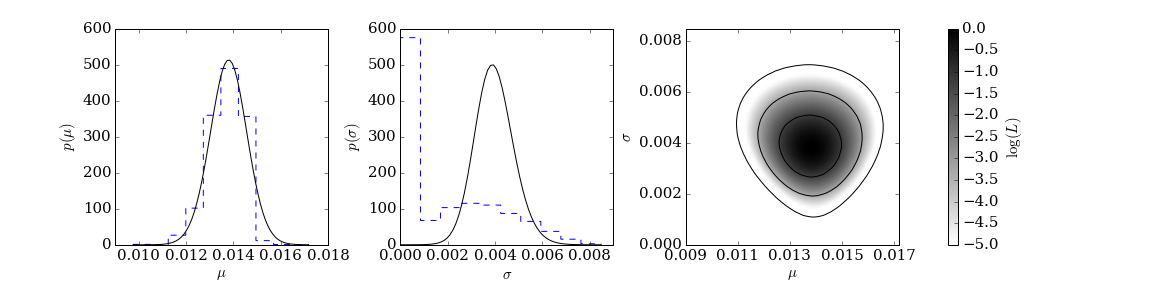
\includegraphics[width=\textwidth]{Fig_5-8_AstroML_obj_217720894888346446_.png}
\cprotect\caption{Two-step approach to finding $\mu$ and $\sigma$ via $\mu_{0}$ and $\sigma_{0}$ for an object 217720894888346446. In this calculation we use raw psf flux, before employing the faint source treatment outlined in Section~\ref{sec:faint_sources}. On the left and middle panels,  solid lines trace marginalized posterior pdfs for $\mu$ and $\sigma$ , while dashed lines depict histogram distributions of 10,000 bootstrap resamples for $\mu_{0}$ and $\sigma_{0}$. The right panel shows the logarithm of the posterior probability density function for $\mu$ and $\sigma$.}
\end{figure*}

On Fig.~\ref{fig:sigma_example} we plot the stages of calculating $\mu$ and $\sigma$. Left and middle panels compare the two methods of calculating variability parameters. The initial approximation (dashed) is based on bootstrapped resampling of ($x_i$, $e_i$) points from  the lightcurve. By randomly resampling the lightcurve $M$ times, instead of a single sample with $N \approx 10-70 $ points  we have $M$ samples. The histogram of  $M=1000$ values for $\mu$, $\sigma$ from resampling is plotted with dashed lines. 
We use the approximate values to provide bounds for the $200 x 70$ grid of $\mu$, $\sigma$, used to evaluate the full posterior likelihood density function (right panel). This ensures that, despite using a coarse grid to improve computational speed,  we still resolve the peak of the underlying distribution. 
%Note that $\mu_{approx}$ traces well the full solution, but $\sigma_{approx}$ has a pile-up torawds 0, due to ... 


\begin{figure*}
\label{fig:lc_example_seasonal}
 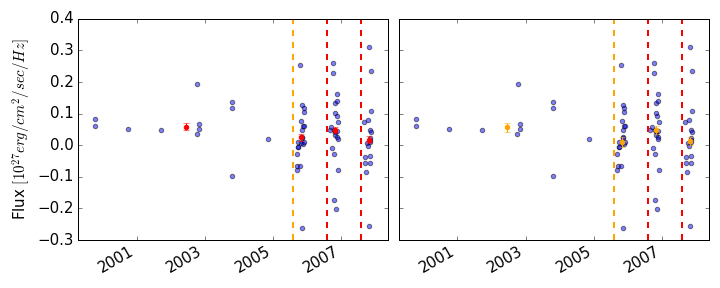
\includegraphics[width=\textwidth]{Lightcurve_full_seasonal_obj_217720894888346425.png}
 \cprotect\caption{A plot showing an outcome of seasonal averaging for an object id 217720894888346425. The left panel (red dots) shows  (mean, meanErr),  and the right panel (orange) shows (median,medianErr), instead of seasonal points (blue). Vertical dashed lines as on Fig.~\ref{fig:lc_example}}
\end{figure*}

%\subsubsection{Variable Candidates Selection}

%
%%%%%%%%%%%%%%%%% TO WHAT DATA WE CALCULATE STATS  %%%%%%%%%%%%%%%%%
%

%
% FIRST SWIPE : FULL LIGHTCURVES 
%

%
% DEFINITION OF VARIABILITY 
% 
All variability parameters describe in a certain way the lightcurve variability. $\sigma_{full}$  corresponds to the spread of the flux distribution. For a non-variable source, $\chi^{2}$ would be centered about 1, with a width $\sigma$ of $\sqrt{2/N}$, where $N$ is the number of points per lightcurve. Thus we would expect that for any distribution $50\%$ of sources would have $\chi^{2}>1$. Therefore a $"3\sigma"$ variability detection would require $\chi^{2} > \chi^{2}_{limit}$, with $\chi^{2}_{limit} = 1 + 3\sqrt{2/N}$
We call a source a 'robust variability candidate' if $\sigma_{full}>0$ and ($\chi^{2}_{DOF} > \chi^{2}_{limit}$ or $\chi^{2}_{R} > \chi^{2}_{limit}$), i.e. we require the full $\sigma$ to be larger than 0, and either robust or DOF $\chi^{2}$ to be larger than the limiting $\chi^{2}$. 

%
% DEFINITION OF A SEASON
% 

%\subsubsection{Seasonal Statistics}
Initially, we evaluate variability parameters $\mu_{full}$, $\sigma_{full}$, $\chi^{2}_{dof}$, and $\chi^{2}_{R}$ based on all points of the lightcurve. Only for variable sources, as defined above, we calculate the variability parameters for the seasonally-binned portions of the lightcurve. The $\chi^{2}_{DOF}$ vs. $\chi^{2}_{R}$ plotted on Fig. ...  shows that these distributions are similar for seasons as well as full lightcurves.    

%
% SECOND SWIPE : SEASONS AND SEASONALLY-BINNED LIGHTCURVES 
% 



\subsubsection{Colors}
%
%%%%%%%%%%%%%%%%% WHY WE NEED COLORS  %%%%%%%%%%%%%%%%%
%


%
%%%%%%%%%%%%%%%%% OUR CONVENTION ON CALCULATING MAGNITUDES  %%%%%%%%%%%%%%%%%
%


%
%%%%%%%%%%%%%%%%% EXTINCTION CORRECTION  %%%%%%%%%%%%%%%%%
%

%\subsection{Extinction Correction}
Since the reported fluxes are not extinction-corrected, we use a table of E(B-V) in a direction of a given source to correct for the galactic extinction. We use the formula  $x_{corr}  = x_{obs} + A_{x} * E(B-V)$, where $x$ is  u,g,r,i,z , and $A_x$ is 5.155, 3.793, 2.751, 2.086, 1.479  for each filter respectively  [Schlegel 98, Av are for RV = 3.1, also suggested by Eddie Schlafly] 




\begin{figure}
\label{fig:coadds_ext}
 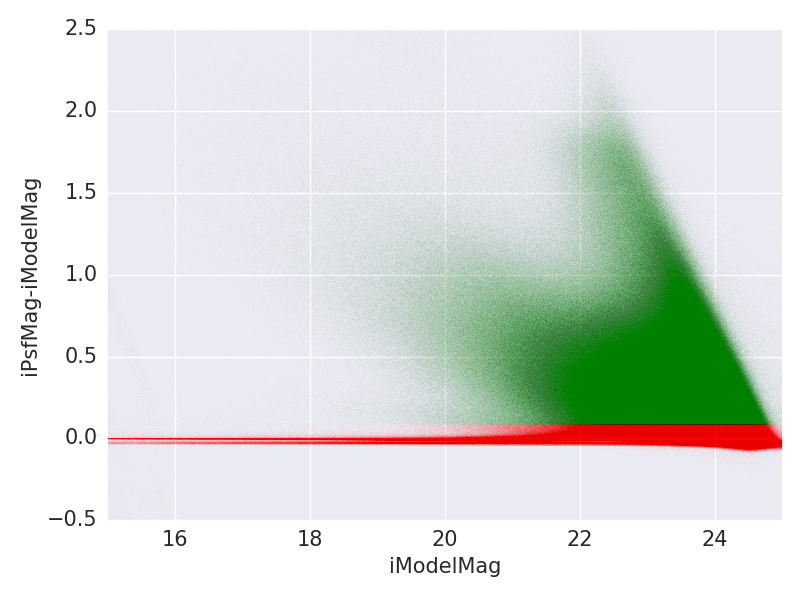
\includegraphics[width=\columnwidth]{Extendedness_coadd_data_16520093_srcs_lim.png}
 \cprotect\caption{A plot showing NCSA sources detected in coadds, removing the outliers beyond the edges of the plot. The coloring corresponds to the \verb|extendedness | parameter calculated in the pipeline based on the iPsfMag-iModelMag : red being 0 (compact), and green being 1 (extended). As iModelMag increases, the separation becomes less certain, as more distant galaxies are more compact.  }
\end{figure}
% 
%\subsection{Photometric colors}

Colors $x-y$ for an object with observations over many epochs are defined as the difference in magnitudes $m_{x} - m_{y}$. To find $m_{x}$, we need to define the average brightness of an object in  a given filter. With a special treatment of faint sources, substituting ($F_{obs}$,$\sigma_F$) for each faint observation by ($<F_{exp}>$,$rms$), we analyse updated lightcurves, addressing sparse sampling (see Fig.~\ref{fig:lc_example}).  

\begin{figure}
\label{fig:lc_example}
 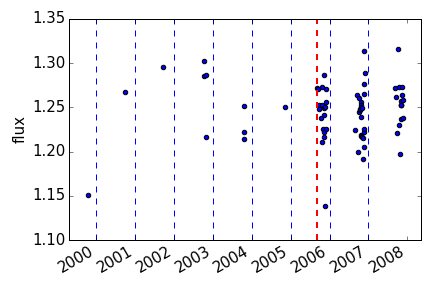
\includegraphics[width=\columnwidth]{Lightcurve_full_obj_217720894888346422.png}
 \cprotect\caption{A plot showing an example lightcurve for an object id 217720894888346422. Jan 1st of each year (blue),  August 1st of 2005 (orange) and August 1st of each subsequent year (red) is indicated by vertical dashed lines. Observations prior to August 1st of 2005 have sparser cadence, whereas those after that date have more frequent observations.  This is due to the SDSS-III Supernova Survey which begun  Sept 1st 2005.  All points to the left of August 1st 2005 (orange line) are averaged together.  Points to the right of August 1st 2005 are seasonally averaged. }
\end{figure}

Thus for a given object we average all sparser observations prior before SDSS-III, and calculate annual averages for all subsequent years. We calculate weighted mean and the rms as 
\begin{equation}
<F> = \frac{\sum {w_{i}F_{i}}}{\sum{w_{i}}} \\
\sigma_{<F>} = \left( \sum{w_{i}}\right) ^{-1/2} 
\end{equation}

with weights as  $w_{i} = 1 / \sigma_{i}^{2}$. We also calculate the robust  median and the median error : $\sqrt{\pi / 2} \, \sigma_{F}$  [ robust $\sigma_{G} = 0.7414 * (75\% - 25\%) $ , based on the interquartile range] . Then lightcurve for a given object is reduced to one ($F_{i}, \sigma_{i}$) point prior to March 2006, and a single point per every subsequent year, where  ($F_{i}, \sigma_{i}$) is ($mean$, $meanErr$) or ($median$, $medianErr$).


The resulting average flux is converted to magnitude, and the color is  $c = m_{x}-m_{y}$, with combined errors of band lightcurves added in quadrature




\section{Results}
\label{sec:results}


\begin{figure*}
\label{fig:colors_example}
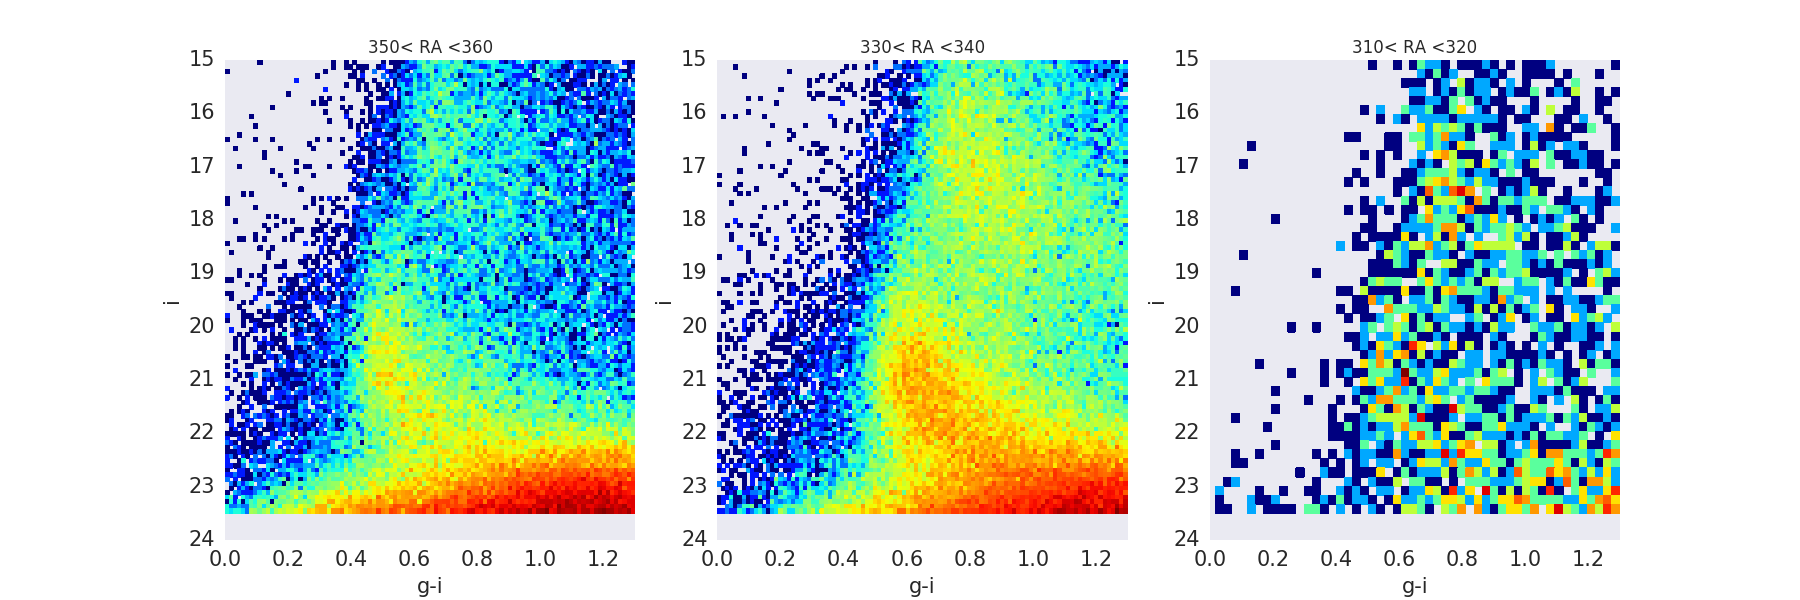
\includegraphics[width=\textwidth]{Fig_g-i_vs_i_ra_310-360hist_n_50row_ext_0.png}
\cprotect\caption{A color-magnitude plot , reproducing the results of Sesar+2010 , Fig.23 .  We show here only NCSA-processed sources, which is why certain RA ranges are omitted or have less sources. We only select sources with \verb|extendedness=0| parameter (stars).  The scale is showing the $\log_{10}$ of count. All sources have their  colors corrected for extinction. On first two panels the features of Sagittarius Stream are clearly visible. }
\end{figure*}
% 



% http://tex.stackexchange.com/questions/3173/how-to-make-a-figure-span-on-two-columns-in-a-scientific-paper 
\begin{figure*}
\label{fig:coadds_ext_hist}
 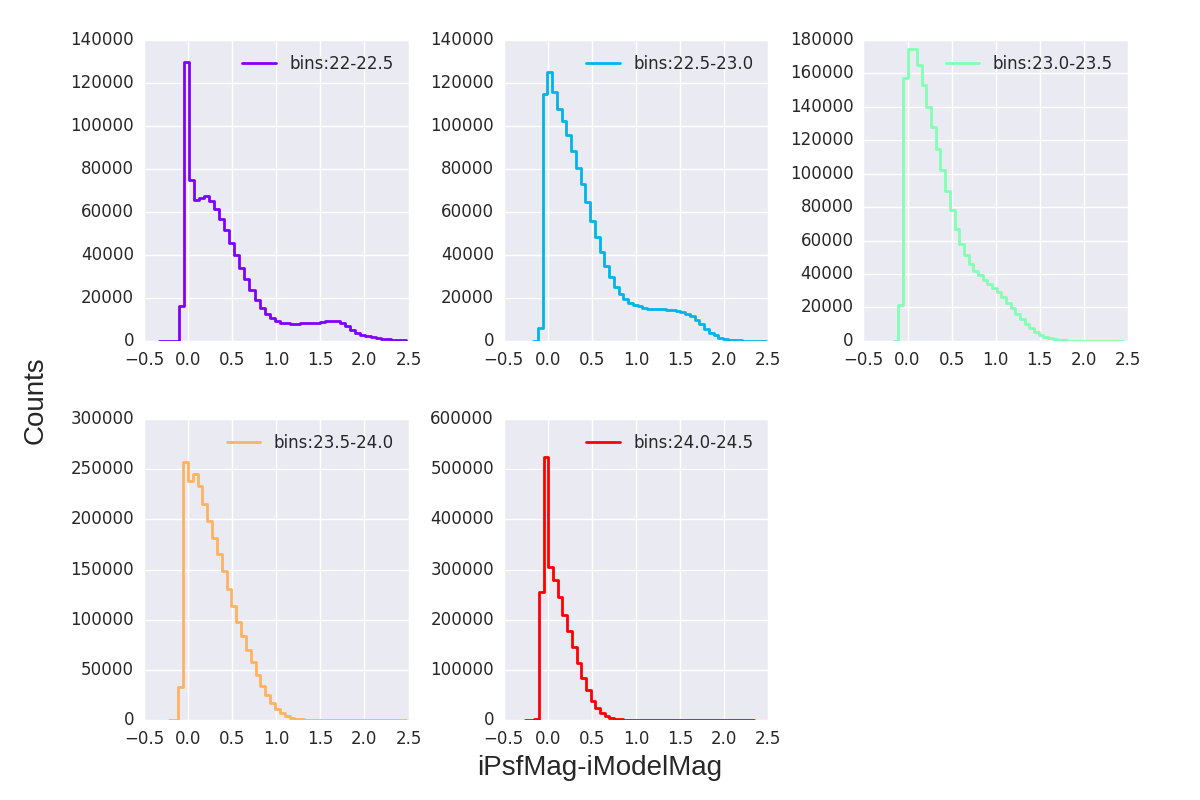
\includegraphics[width=\textwidth]{Extendedness_coadd_histograms.png}
 \caption{The histograms show the count of sources in 5 magnitude bins, corresponding to the vertical cut through Fig.~\ref{fig:coadds_ext}. It helps to verify how well can the extended and compact sources be separated based solely on the iPsfMag-iModelMag}
\end{figure*}






\section{Conclusions}
\label{sec:conclusions}



\section*{Acknowledgements}

Funding for the SDSS and SDSS-II has been provided by the Alfred P. Sloan Foundation, the Participating Institutions, the National Science Foundation, the U.S. Department of Energy, the National Aeronautics and Space Administration, the Japanese Monbukagakusho, the Max Planck Society, and the Higher Education Funding Council for England. The SDSS Web Site is http://www.sdss.org/.

The SDSS is managed by the Astrophysical Research Consortium for the Participating Institutions. The Participating Institutions are the American Museum of Natural History, Astrophysical Institute Potsdam, University of Basel, University of Cambridge, Case Western Reserve University, University of Chicago, Drexel University, Fermilab, the Institute for Advanced Study, the Japan Participation Group, Johns Hopkins University, the Joint Institute for Nuclear Astrophysics, the Kavli Institute for Particle Astrophysics and Cosmology, the Korean Scientist Group, the Chinese Academy of Sciences (LAMOST), Los Alamos National Laboratory, the Max-Planck-Institute for Astronomy (MPIA), the Max-Planck-Institute for Astrophysics (MPA), New Mexico State University, Ohio State University, University of Pittsburgh, University of Portsmouth, Princeton University, the United States Naval Observatory, and the University of Washington. 

\appendix
\section{\\ Treatment of faint sources}
\label{App:AppendixA}

In our calculations we used the  \verb|scipy| implementation of 
the following often used integrals of Gaussian distributions : 

- cumulative density function, that is an area under the Gaussian distribution from $-\infty$ to $x_{0}$ :

\begin{equation}
\cdf(x_{0}) = \int_{-\infty}^{x_{0}}{\mathcal{N}(\mu,\sigma)dx} = \int_{-\infty}^{x_{0}}{\frac{\exp{(x-\mu)^{2} / 2\sigma^{2}}}{\sqrt{2\pi\sigma^{2}}} dx}
\end{equation}

- point percent function , that is an inverse of the cumulative density function:  if  $A = \cdf(x_{0})$, then  $x_{0} = \ppf(A)$

- survival function (also known  as the complementary cumulative distribution function), that is an area under a Gaussian distribution from $x_{0}$ to $\infty$

\begin{multline}
\sf(x_{0}) =  \int_{x_{0}}^{\infty}{\mathcal{N}(\mu,\sigma)dx} =  \int_{-\infty}^{\infty}{\mathcal{N}(\mu,\sigma)dx} -  \int_{-\infty}^{x_{0}}{\mathcal{N}(\mu,\sigma)dx} = \\
1 - \cdf(x_{0})
\end{multline}

In our faint flux treatment  we assume that each flux measurement has an associated Gaussian likelihood, and that the width and mean of the likelihood correspond 
to the measured flux and the measurement error respectively. 

For a source where signal-to-noise < 2 (in our case, ratio of  flux to error), we remove the negative portion of the likelihood, since there is no physical likelihood that a flux would be negative.
Thus for mean, we integrate from $0$ instead of $-\infty$ : 


\begin{equation}
F_{mean} = \frac{\int _{0} ^ {\infty}{F p(F) dF}}{\int _{0} ^ {\infty}{p(F) dF}} = I_{0} / I_{1}
\end{equation}

where we need to normalize by the integral over the positive part of the Gaussian likelihood. 

We evaluate 

\begin{multline}
I_{0}= \int _{0} ^ {\infty} {\frac{F}{\sqrt{2\pi\sigma_{F}^{2}}} \exp{\left(-\frac{(F-F_{obs})^{2}}{2\sigma_{F}^{2}}\right)} }dF = \\  \frac{\sigma_{F}}{\sqrt{2 \pi}} \exp{\left(- \frac{F_{obs}^{2}}{2\sigma_{F}^{2}} \right)} + F_{obs} \sf{\left( \frac{-F_{obs}}{\sigma_{F}}\right)}
\end{multline}

and 

\begin{equation}
I_{1} = \int _{0} ^ {\infty}{ p(F) dF} = \int _{0} ^ {\infty} {\frac{\exp{\left(-\frac{(F-F_{obs})^{2}}{2\sigma_{F}^{2}}\right)} }{\sqrt{2\pi\sigma_{F}^{2}}} }dF = \sf{(-F_{obs} / \sigma_{F})}
\end{equation}

so that 
\begin{equation}
x_{mean} = \frac{\exp{(- x_{obs}^{2} / 2 )} }{\sf{(-x_{obs})}\sqrt{2 \pi}} + x_{obs} 
\end{equation}

where we scaled $F_{obs}$ by  $\sigma_F$  (i.e. $F_{mean} = x_{mean} \cdot \sigma_{F}$). 



\bigskip

To find the median and the $2\sigma$ level we transform from $F$ space to $x$ space , scaling by  $\sigma_{F}$, so that $x = F / \sigma_{F}$ , and thus the likelihood $p(x) \sim \mathcal{N}(x_{obs},1)$ is :
\begin{equation}
p(x) = \frac{1}{\sqrt{2  \pi }} \exp{ \left(-\frac{(x-x_{obs})^{2}}{2}\right)}
\end{equation}

We  then transform from $x$ to $z$ space, with  a translation by $x_{obs} = F_{obs} / \sigma_{F}$ :  $z = x - x_{obs}$  , so that now  $p(z) \sim \mathcal{N}(0,1)$:
\begin{equation}
p(z) = \frac{1}{\sqrt{2  \pi }} \exp{ \left(-\frac{z^2}{2}\right)}
\end{equation}



In $z$-space, the median from 

\begin{equation}
\int_{0}^{x_{med}} {p(x)dx} = \int_{x_{med}}^{\infty} {p(x)dx}
\end{equation}
 
becomes 

\begin{equation}
\int_{x_{0}}^{z_{med}}{p(z)dz} = \int_{z_{med}}^{\infty}{p(z)dz}
\end{equation}

with  $x_{0}=-x_{obs}$

\bigskip

We evaluate $z_{med}$ analytically  - the right hand side is the survival function  : 

\begin{equation}
\int_{z_{med}}^{\infty}{p(z)dz} = \sf(z_{med})
\end{equation}

and the left hand side, assuming that the median $z_{med} > x_{0}$, is :

\begin{multline}
\int_{x_{0}}^{z_{med}}{p(z)dz} = \int_{-\infty}^{z_{med}}{p(z)dz} - \int_{-\infty}^{x_{0}}{p(z)dz} = \cdf(z_{med}) - \cdf(x_{0})
\end{multline}

Rearranging, and using the percent point function ($\ppf$)  we find:

\begin{equation}
z_{med} = \ppf \left( \frac{1+\cdf(x_{0})}{2} \right)
\end{equation}

and transforming back to $F$ space: 

\begin{equation}
F_{med} = F_{obs} + \sigma_{F} \, \ppf \left( \frac{1+\cdf(x_{0})}{2} \right)
\end{equation}

with $x_{0}$ and $x_{obs}$ as above.  We also normalize this expression by $\int _{0} ^ {\infty}{ p(F) dF}$ and $\sigma_{F}$:

\begin{equation}
x_{med}^{norm} = x_{obs}
\end{equation}


\bigskip

In $z$  space , the $2\sigma$ areas  $A$ and $B$ are :

$\text{A} = \sf(x_{0})$ and $\text{B} = \sf(z_{B})$, so to find  $z_{B}$ we use the  inverse survival function $\isf$ : $z_{B} = \isf(0.05 \text{A})$. Thus transforming back to $F$-space we have:

\begin{equation}
F_{2\sigma} = F_{obs} + \sigma_{F} \left(\, \isf (\, 0.05 \sf (x_{0})  \right)
\end{equation}

\bigskip

We also find the root-mean-square:

\begin{equation}
F_{rms}^{2} = \frac{\int _{0} ^ {\infty}{(F-F_{mean})^{2} p(F) dF}}{\int _{0} ^ {\infty}{p(F) dF}} = I_{0} / I_{1}
\end{equation}

this can be evaluated by numerical integration, scaling by $\sigma_{F}$, so that $x_{mean} = F_{mean} / \sigma_{F}$, $x_{obs} = F_{obs} / \sigma_{F}$ : 

\begin{equation}
F_{rms}^{2} = \frac{\sigma_{F}^{2} \int_{0}^{\infty} {(x-x_{mean})^{2} exp(-(x-x_{obs})^{2} / 2 ) dx }}  {\int_{0}^{\infty} {exp(-(x-x_{obs})^{2} / 2 ) dx }}
\end{equation}

We derived analytical expression for rms :
\begin{equation}
x_{rms} = \left(\frac{I_{0}}{I_{1} \sigma_{F}^{2}}\right)^{1/2}
\end{equation}

where $I_{1}$ is our normalization , as in calculation of $F_{mean}$, and as 


\begin{equation}
\frac{I_{0}}{ \sigma_{F}^{2}} = \frac{1}{2} \erf\left(\frac{x_{obs}}{\sqrt{2}}\right) + \frac{1}{\sqrt{2\pi}} e^{(-x_{obs}^{2} / 2)} (2 \Delta x - x_{obs}) + (\Delta x)^{2} \sf(-x_{obs})
\end{equation}
with  $\Delta x = x_{obs} - x_{mean}$

\section{\\ Characterizing variability}
\label{App:AppendixB}


We further characterize the variability of lightcurves by calculating $\sigma_{0}$ (the approximate value), and $\sigma_{full}$, following Ivezic+2014, chapter 5. 

$\sigma_{0}$ is found in the following way: if by ($x_{i}, e_{i}$) we denote the measurement and associated error, then the bootstrapped sampling of ($x_{i}, e_{i}$) is sampling each vector at a number of N random indices (eg. N=1000). Thus instead of $x_{i}$ which may include only N=10 measurements, we have $x_{i,boot}$ which has N=1000 random samples. Median is the 50-th percentile of any sample.  Following [Ivezic+2014], chapter 5, we use the sample median to estimate $\mu_{0} = median(x_{i,boot})$, and an interquartile range width estimator to estimate the standard deviation : $\sigma_{G} =0.7413 (X_{75\%} - X_{25\%}) $ for $X = x_{i,boot}$.
With the median error $e_{50} = median(e_{i,boot})$, we estimate $\sigma_{0}$ as : 

\begin{equation}
\sigma_{0} = ( variance_{approx} )^{1/2} = (\zeta^{2} \cdot \sigma_{G}^{2} - e_{50} ^ {2})^{1/2}
\end{equation}

where 

\begin{equation}
\zeta = \frac{median(\widetilde{\sigma}_{i})} {mean(\widetilde{\sigma}_{i})}
\end{equation}

and 

\begin{equation}
\widetilde{\sigma}_{i} =  ( \widetilde{variance} )^{1/2} = ( \sigma_{G}^{2} + e_{i}^{2} - e_{50}^{2} )^{1/2}
\end{equation}


For the marginalized $\sigma_{full}$, we calculate logarithm of the posterior probability distribution for the grid of $\mu$ and $\sigma$ values as:

\begin{equation}
\log{L} = -0.5 \sum \left( \ln(\sigma^{2}+e_{i}^{2}) + \frac{(x_{i}-\mu)^{2}}{(\sigma^{2}+e_{i}^{2})} \right)
\end{equation}

We shift the maximum value of logL by subtracting the maximum value of logL, thus calculating the likelihood : 

\begin{equation}
L = e^{\log{L} - max(\log{L})}
\end{equation}

We then marginalize over $\mu$ or $\sigma$ : 

\begin{equation}
p(\sigma) = \sum_{\mu}(L_{\sigma,\mu}) \\
p(\mu) = \sum_{\sigma}(L_{\sigma,\mu})
\end{equation}

and normalize the probability :

\begin{equation}
p_{norm}(\sigma) = \frac{p(\sigma)}{ \int {p(\sigma) \text{d}\sigma}} \\ 
p_{norm}(\mu) = \frac{p(\mu)} {\int {p(\mu) \text{d}\mu} }
\end{equation}


To characterize  lightcurve variability we first calculate for the entire lightcurve of an object  the approximate $\mu_{0}$ and $\sigma_{0}$ using bootstrapped resampling of the lightcurve.  This yields the boundaries for the more exact calculation of the full 2D log-likelihood performed on a grid of $\mu$ and $\sigma$ values. Thus the more accurate $\sigma_{full}$ and $\mu_{full}$ are found as a maximum of the 2D log-likelihood distribution (see Fig.~\ref{fig:sigma_example} ).



\section{\\ Making of ugriz metrics }
\label{App:AppendixC}

Colors can be calculated in two ways: using the median of forced photometry over all epochs (object detected in coadded i-band has photometry in all epochs:  \verb|ugrizMetrics.csv|), or the median over single-epoch detections (only when an object was above the detection threshold for a single epoch : \verb|medianPhotometry.csv|).  
The median over all detections will be biased (especially for faint sources) towards higher brightness.  On the other hand, the median over all epochs will be more representative of the true brightness of an object in a given filter.  If a median brightness is negative, we can use zero point magnitudes and in such cases median over all epochs will be an upper limit on brightness, but still less biased than median over all detections. Therefore  we choose to use median over all epochs to calculate colors (see Fig.~\ref{fig:colors_example} for an example).  

\section{\\ Zero Flux Magnitudes }
\label{App:AppendixD}

If the median flux of an object over all epochs  is negative (an outcome of forced photometry on fluctuating noise), we cannot define its magnitude in that filter.  In such situation one can revert to  using for each negative flux the zero point magnitude ($m_1$) - the magnitude for a source with a flux of 1 count per sec, different for each exposure.  The zero point magnitude for each exposure with negative flux is calculated from the  Flux of 0 magnitude source,  $F_0$,  as  $m_{1} = 2.5 \log_{10}{F_{0}}$. For that object the new median magnitude in that filter will be the upper limit. We did not use this method, since a better way is to calculate the $2-\sigma$ flux limit for each flux measurement $< 2 \sigma$ : $F_{2\sigma}$. 

\section{\\ Lightcurve Metrics}
For each object we calculate lightcurve-derived metrics. Denoting \verb|psfFlux| and \verb|psfFluxErr| as $y$ and $\sigma_{y}$, we find the number of measurements per lightcurve (N), the mean flux, the median flux (the 50th quartile), median flux error \verb|e50|, mean flux error \verb|e_mean|, $\sigma_{G}$ (based on interquartile flux range 0.7413(q75-q25)), $\chi^{2}$:
\begin{equation}
\frac{1}{N-1} \sum{\left( \frac{y-mean(y)}{\sigma_{y}} \right) ^{2}}
\end{equation}
 mean weighted by the \verb|WVar| - the inverse variance (\verb|WeightedMean|), and the standard deviation weighted by inverse variance and corrected for intrinsic scatter (\verb|WeightedStdCorr|):

\begin{equation}
\mbox{WVar} = \left( \sum{\frac{1}{\sigma_{y}^{2}}} \right) ^{-1}
\end{equation} 

\begin{equation}
\mbox{WeightedMean} = \mbox{WVar} \sum{\frac{y}{\sigma_{y}^{2}}}
\end{equation}

\begin{equation}
\mbox{WeightedStdCorr} =  \left[ \frac{ \mbox{WVar}  }{N-1} \sum{\frac{(y-\mbox{WeightedMean})^{2}}{\sigma_{y}^{2}}} \right] ^{1/2}
\end{equation}



From these metrics, we can calculate the catalog photometry  :

\begin{equation}
\verb|median_mag| = -2.5 \log_{10}\mbox{median} - 48.6
\end{equation}

There are  $5892054$ sources with catalog photometry brighter than $23$ mag  (\verb|ugrizMetrics.csv|). 

We can also calculate median photometry over all individual epochs  detections, cross-matched by extinction tables [HOW ? ]  There are $12373162$ sources with median photometry, matched with E(B-V) data (\verb|medianPhotometry.csv|) . 

For each band we calculate metrics describing the lightcurve behavior for a given band, including the Butler \& Bloom classifier, which can  for high S/N objects, where it has a good discriminating power. It's advantage over the full DRW analysis for each lightcurve is that by assuming a range of $\tau$, amplitude, expected for a DRW for a QSO, we calculate the likelihood of a given lightcurve belonging to a QSO ( \verb|i_metrics.csv|). 


%%%%%%%%%%%%%%%%%%%%%%%%%%%%%%%%%%%%%%%%%%%%%%%%%%

%%%%%%%%%%%%%%%%%%%% REFERENCES %%%%%%%%%%%%%%%%%%

% The best way to enter references is to use BibTeX:

%\bibliographystyle{mnras}
%\bibliography{example} % if your bibtex file is called example.bib

%%%%%%%%%%%%%%%%%%%%%%%%%%%%%%%%%%%%%%%%%%%%%%%%%%


% Don't change these lines
\bsp	% typesetting comment
\label{lastpage}
\end{document}

% End of mnras_template.tex
